% Part 1: Medium Problems (6 problems)
% These problems combine 2-3 mathematical topics with sophisticated reasoning

% Problem 1: AM-GM Optimization (Sample 01)
\begin{problem}[AM-GM Surface Area Optimization]
(a) Prove that for positive real numbers $x, y, z$:
\[ \frac{1}{x} + \frac{1}{y} + \frac{1}{z} \ge \frac{3}{\sqrt[3]{xyz}} \]

(b) A rectangular prism has dimensions $a, b, c$ and a fixed, constant Volume $V$.
Using part (a), show that the Total Surface Area $S$ is minimized when the prism is a cube.

\vspace{1cm}

\begin{center}
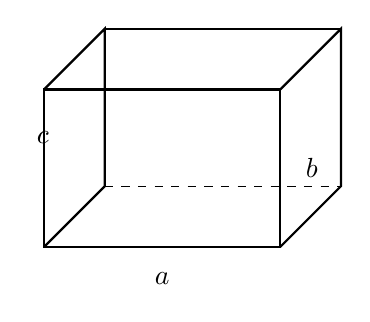
\begin{tikzpicture}[scale=2]
    % Draw Cuboid
    \draw[thick] (0,0,0) -- (1.5,0,0) -- (1.5,1,0) -- (0,1,0) -- cycle;
    \draw[thick] (0,0,0) -- (0,0,-1) -- (0,1,-1) -- (0,1,0);
    \draw[thick] (1.5,0,0) -- (1.5,0,-1) -- (1.5,1,-1) -- (1.5,1,0);
    \draw[thick] (0,1,-1) -- (1.5,1,-1);
    \draw[dashed] (0,0,-1) -- (1.5,0,-1);
    
    % Labels
    \node at (0.75, -0.2, 0) {$a$};
    \node at (1.7, 0.5, 0) {$b$};
    \node at (-0.2, 0.5, -0.5) {$c$};
\end{tikzpicture}
\end{center}
\end{problem}

\begin{hint}
For part (a), apply AM-GM inequality directly to the reciprocals $\frac{1}{x}, \frac{1}{y}, \frac{1}{z}$. For part (b), express the surface area $S = 2(ab + bc + ca)$ in terms of the volume constraint $V = abc$, then use part (a) with strategic substitution.
\end{hint}

\begin{solution}
\textbf{(a) Proof:}
Since $x, y, z > 0$, then $\frac{1}{x}, \frac{1}{y}, \frac{1}{z} > 0$.
Applying the AM-GM inequality to these three terms:
\begin{align*}
    \frac{\frac{1}{x} + \frac{1}{y} + \frac{1}{z}}{3} &\ge \sqrt[3]{\frac{1}{x} \cdot \frac{1}{y} \cdot \frac{1}{z}} \\
    \frac{1}{x} + \frac{1}{y} + \frac{1}{z} &\ge 3 \sqrt[3]{\frac{1}{xyz}} \\
    \frac{1}{x} + \frac{1}{y} + \frac{1}{z} &\ge \frac{3}{\sqrt[3]{xyz}}
\end{align*}

\textbf{(b) Application:}
Let the dimensions be $a,b,c$.
\begin{itemize}
    \item Fixed Volume: $V = abc$ (constant).
    \item Surface Area: $S = 2(ab + bc + ca)$.
\end{itemize}

We want to relate $S$ to the reciprocals in part (a).
\begin{align*}
    S &= 2abc \left( \frac{1}{c} + \frac{1}{a} + \frac{1}{b} \right) \\
    S &= 2V \left( \frac{1}{a} + \frac{1}{b} + \frac{1}{c} \right)
\end{align*}
From part (a), we know $\left( \frac{1}{a} + \frac{1}{b} + \frac{1}{c} \right) \ge \frac{3}{\sqrt[3]{abc}}$.
Substituting this into the expression for $S$:
\begin{align*}
    S &\ge 2V \left( \frac{3}{\sqrt[3]{V}} \right) \\
    S &\ge 6 V^{1} V^{-1/3} \\
    S &\ge 6 V^{2/3}
\end{align*}
Since $V$ is constant, $6V^{2/3}$ is a constant minimum value.
Equality holds (minimum $S$ occurs) when the terms in the AM-GM are equal:
\[ \frac{1}{a} = \frac{1}{b} = \frac{1}{c} \implies a = b = c \]
Therefore, the prism is a cube. \hfill $\square$
\end{solution}

\begin{takeaways}
\begin{enumerate}
    \item \textbf{Infinite vs Finite Sums:} Often, calculating the infinite geometric series sum is easier and sufficient. If the infinite sum creates a contradiction ($< 1$), then the finite sum definitely will too.

    \item \textbf{Strict Inequalities:} Geometric series of positive terms are always strictly less than their limit at infinity.
\end{enumerate}
\end{takeaways}

% Problem 2: Vector Ellipsoid (Sample 06)  
\begin{problem}[Cauchy-Schwarz on Ellipsoid]
The point $P(x, y, z)$ lies on the surface of the ellipsoid defined by:
\[ \frac{x^2}{4} + \frac{y^2}{9} + \frac{z^2}{25} = 1 \]
\begin{itemize}
    \item[(i)] By choosing appropriate vectors $\mathbf{u}$ and $\mathbf{v}$ and applying the Cauchy-Schwarz inequality ($\mathbf{u} \cdot \mathbf{v} \le |\mathbf{u}||\mathbf{v}|$), find the maximum value of $x + y + z$.
    \item[(ii)] Find the coordinates of $P$ in the first octant where this maximum occurs.
\end{itemize}

\begin{center}
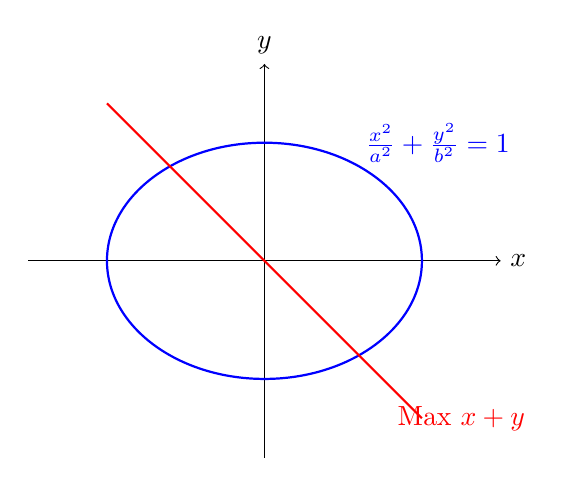
\begin{tikzpicture}
    \draw[->] (-3,0) -- (3,0) node[right] {$x$};
    \draw[->] (0,-2.5) -- (0,2.5) node[above] {$y$};
    \draw[thick, blue] (0,0) ellipse (2cm and 1.5cm);
    \node[blue] at (2.2, 1.5) {$\frac{x^2}{a^2} + \frac{y^2}{b^2} = 1$};
    \draw[red, thick] (-2, 2) -- (2, -2);
    \node[red] at (2.5, -2) {Max $x+y$};
\end{tikzpicture}
\end{center}
\end{problem}

\begin{hintbox}
The standard Cauchy-Schwarz inequality is $|\mathbf{a} \cdot \mathbf{b}| \le |\mathbf{a}| |\mathbf{b}|$.
You cannot define $\mathbf{u} = (x, y, z)$ directly because the sum of squares is not 1.
Instead, define $\mathbf{u}$ such that $|\mathbf{u}|^2$ exactly matches the left-hand side of the ellipsoid equation.
Then, choose a constant vector $\mathbf{v}$ such that the dot product $\mathbf{u} \cdot \mathbf{v}$ recovers the expression $x + y + z$.
\end{hintbox}

\begin{solution}
\textbf{(i)} Let $\mathbf{u} = \begin{pmatrix} \frac{x}{2} \\ \frac{y}{3} \\ \frac{z}{5} \end{pmatrix}$. We are given $|\mathbf{u}|^2 = \frac{x^2}{4} + \frac{y^2}{9} + \frac{z^2}{25} = 1$, so $|\mathbf{u}|=1$.
We want to maximize $x+y+z$. We observe:
\[ x+y+z = \frac{x}{2}(2) + \frac{y}{3}(3) + \frac{z}{5}(5) \]
This suggests setting $\mathbf{v} = \begin{pmatrix} 2 \\ 3 \\ 5 \end{pmatrix}$.
Apply Cauchy-Schwarz:
\[ \mathbf{u} \cdot \mathbf{v} \le |\mathbf{u}| |\mathbf{v}| \]
\[ x + y + z \le (1) \sqrt{2^2 + 3^2 + 5^2} \]
\[ x + y + z \le \sqrt{4 + 9 + 25} = \sqrt{38} \]

\textbf{(ii)} Equality occurs when $\mathbf{u} = k\mathbf{v}$, i.e., $\frac{x}{2} = 2k, \frac{y}{3} = 3k, \frac{z}{5} = 5k$.
So $x=4k, y=9k, z=25k$.
Substitute into the plane eq $x+y+z = \sqrt{38}$:
\[ 4k + 9k + 25k = \sqrt{38} \implies 38k = \sqrt{38} \implies k = \frac{1}{\sqrt{38}} \]
Point $P$: $\left( \frac{4}{\sqrt{38}}, \frac{9}{\sqrt{38}}, \frac{25}{\sqrt{38}} \right)$.
\end{solution}

\begin{takeaways}
\begin{enumerate}
    \item \textbf{Normalization:} If given a constraint like $Ax^2 + By^2 = C$, define vector components as $\sqrt{A}x$ and $\sqrt{B}y$.
    \item \textbf{The "Canceling" Vector:} The second vector is chosen specifically to cancel out the denominators introduced by the normalization step.
\end{enumerate}
\end{takeaways}

% Problem 3: Vector Dot Products (Sample 08)
\begin{problem}[Unit Vector Cosine Sum]
Four unit vectors $\mathbf{v}_1, \mathbf{v}_2, \mathbf{v}_3, \mathbf{v}_4$ originate from the origin $O$.
It is given that their vector sum is zero:
\[ \mathbf{v}_1 + \mathbf{v}_2 + \mathbf{v}_3 + \mathbf{v}_4 = \mathbf{0} \]
Let $\theta_{ij}$ be the angle between vectors $\mathbf{v}_i$ and $\mathbf{v}_j$.
Show that the sum of the cosines of the angles between all distinct pairs is $-2$.
\[ \sum_{1 \le i < j \le 4} \cos \theta_{ij} = -2 \]

\begin{center}
\begin{tikzpicture}[scale=2]
    \draw[->, thick] (0,0) -- (1,0) node[right] {$\mathbf{v}_1$};
    \draw[->, thick] (0,0) -- (-0.5, 0.866) node[above left] {$\mathbf{v}_2$};
    \draw[->, thick] (0,0) -- (-0.5, -0.866) node[below left] {$\mathbf{v}_3$};
    \draw[->, thick] (0,0) -- (0.2, -0.9) node[below right] {$\mathbf{v}_4$};
    \node at (0,0.2) {$O$};
\end{tikzpicture}
\end{center}
\end{problem}

\begin{hintbox}
Consider the squared magnitude of the vector sum.
Since $\sum \mathbf{v}_i = \mathbf{0}$, it follows that $|\sum \mathbf{v}_i|^2 = 0$.
Expand the dot product $(\mathbf{v}_1 + \dots + \mathbf{v}_4) \cdot (\mathbf{v}_1 + \dots + \mathbf{v}_4)$.
Separate the expansion into "self-products" ($\mathbf{v}_i \cdot \mathbf{v}_i$) and "cross-products" ($\mathbf{v}_i \cdot \mathbf{v}_j$).
\end{hintbox}

\begin{solution}
Let $S = \mathbf{v}_1 + \mathbf{v}_2 + \mathbf{v}_3 + \mathbf{v}_4 = \mathbf{0}$.
\[ |S|^2 = S \cdot S = 0 \]
Expanding the dot product:
\[ \sum_{i=1}^4 |\mathbf{v}_i|^2 + 2 \sum_{1 \le i < j \le 4} (\mathbf{v}_i \cdot \mathbf{v}_j) = 0 \]
We are given that vectors are unit vectors, so $|\mathbf{v}_i|^2 = 1$ for all $i=1..4$.
There are 4 such terms.
\[ 4 + 2 \sum_{1 \le i < j \le 4} (\mathbf{v}_i \cdot \mathbf{v}_j) = 0 \]
Using the definition of dot product: $\mathbf{v}_i \cdot \mathbf{v}_j = |\mathbf{v}_i| |\mathbf{v}_j| \cos \theta_{ij} = 1 \cdot 1 \cdot \cos \theta_{ij}$.
\[ 4 + 2 \sum_{1 \le i < j \le 4} \cos \theta_{ij} = 0 \]
\[ 2 \sum \cos \theta_{ij} = -4 \]
\[ \sum_{1 \le i < j \le 4} \cos \theta_{ij} = -2 \]
\end{solution}

\begin{takeaways}
\begin{enumerate}
    \item \textbf{Squaring the Sum:} The most powerful tool for analyzing vector sums equal to zero (equilibrium) is to take the dot product of the sum with itself.
    \item \textbf{Counting Terms:} When expanding $(\sum_{i=1}^n a_i)^2$, there are $n$ squared terms and $n(n-1)$ cross terms. Since dot product is commutative, this groups into $n$ squared terms and $2 \times (\text{distinct pairs})$.
\end{enumerate}
\end{takeaways}

% Problem 4: Complex Triangle (Sample 11)
\begin{problem}[Complex Numbers Forming Triangle]
Three complex numbers $z_1, z_2, z_3$ satisfy:
\[
\begin{cases}
    |z_1| = |z_2| = |z_3| = r & (r > 0) \\
    z_1 + z_2 + z_3 = 0
\end{cases}
\]
Show that $z_1, z_2, z_3$ represent the vertices of an equilateral triangle inscribed in the circle $|z|=r$.
\end{problem}

\begin{hintbox}
To prove a triangle is equilateral, you can prove the sides are equal: $|z_1-z_2|^2 = |z_2-z_3|^2 = |z_3-z_1|^2$.
Expand $|z_1-z_2|^2 = (z_1-z_2)(\overline{z_1}-\overline{z_2})$.
Use the fact that $z_1+z_2+z_3=0 \implies z_1+z_2 = -z_3$.
\end{hintbox}

\begin{solution}
Consider the squared side length $|z_1 - z_2|^2$:
\begin{align*}
    |z_1 - z_2|^2 &= (z_1 - z_2)(\bar{z}_1 - \bar{z}_2) \\
    &= z_1\bar{z}_1 + z_2\bar{z}_2 - z_1\bar{z}_2 - z_2\bar{z}_1 \\
    &= r^2 + r^2 - (z_1\bar{z}_2 + z_2\bar{z}_1) \\
    &= 2r^2 - 2\text{Re}(z_1\bar{z}_2)
\end{align*}
Now consider the condition $(\sum z)(\sum \bar{z}) = 0 \cdot 0 = 0$.
\[ |z_1|^2 + |z_2|^2 + |z_3|^2 + (z_1\bar{z}_2 + \text{others}) = 0 \]
\[ 3r^2 + (z_1\bar{z}_2 + z_2\bar{z}_1) + \dots = 0 \]
Alternatively, simplify the algebra:
Since $z_1 + z_2 = -z_3$, squaring modulus:
$|z_1+z_2|^2 = |-z_3|^2 \implies |z_1+z_2|^2 = r^2$.
Using the parallelogram law $|z_1+z_2|^2 + |z_1-z_2|^2 = 2(|z_1|^2+|z_2|^2)$:
\[ r^2 + |z_1-z_2|^2 = 2(r^2 + r^2) \]
\[ |z_1-z_2|^2 = 3r^2 \]
By symmetry, $|z_2-z_3|^2 = 3r^2$ and $|z_3-z_1|^2 = 3r^2$.
Since all sides are equal ($\sqrt{3}r$), the triangle is equilateral.
\end{solution}

\begin{takeaways}
\begin{enumerate}
    \item \textbf{Vector Addition:} $z_1+z_2+z_3=0$ means the centroid is the origin. If the circumcenter (origin) and centroid coincide, the triangle is equilateral.
    \item \textbf{Modulus Algebra:} Using $|z_1+z_2|^2 = |-z_3|^2$ is much faster than expanding everything.
\end{enumerate}
\end{takeaways}

% Problem 5: Parametric Motion (Sample 29)
\begin{problem}[Minimum Distance Between Moving Particles]
Two particles $A$ and $B$ move in space such that their position vectors at time $t \ge 0$ are:
\[ \mathbf{r}_A = \begin{pmatrix} 1 \\ 0 \\ 2 \end{pmatrix} + t \begin{pmatrix} 1 \\ 1 \\ 0 \end{pmatrix} \quad \text{and} \quad \mathbf{r}_B = \begin{pmatrix} 4 \\ 2 \\ 0 \end{pmatrix} + t \begin{pmatrix} 0 \\ 1 \\ 1 \end{pmatrix} \]

(i) Express the squared distance $S(t) = |\mathbf{r}_A - \mathbf{r}_B|^2$ as a quadratic in $t$.

(ii) Find the minimum distance between the particles and the time at which this occurs.
\end{problem}

\begin{hintbox}
Find the displacement vector $\mathbf{d}(t) = \mathbf{r}_A - \mathbf{r}_B$.
Compute the dot product $\mathbf{d} \cdot \mathbf{d}$ to get the squared magnitude.
You will get a quadratic expression $At^2 + Bt + C$. Find the vertex of this parabola ($t = -B/2A$).
\end{hintbox}

\begin{solution}
\textbf{(i)} The vector connecting them is:
\[ \mathbf{d} = \mathbf{r}_A - \mathbf{r}_B = \begin{pmatrix} 1-4 \\ 0-2 \\ 2-0 \end{pmatrix} + t \begin{pmatrix} 1-0 \\ 1-1 \\ 0-1 \end{pmatrix} = \begin{pmatrix} -3+t \\ -2 \\ 2-t \end{pmatrix} \]
Squared distance:
\[ S(t) = (-3+t)^2 + (-2)^2 + (2-t)^2 \]
\[ S(t) = (t^2 - 6t + 9) + 4 + (t^2 - 4t + 4) \]
\[ S(t) = 2t^2 - 10t + 17 \]

\textbf{(ii)} To minimize $S(t)$, find $S'(t) = 4t - 10$.
Set $4t - 10 = 0 \implies t = 2.5$.
Substitute $t=2.5$ back into $S(t)$:
\[ S(2.5) = 2(6.25) - 25 + 17 = 12.5 - 25 + 17 = 4.5 \]
Minimum distance = $\sqrt{4.5} = \sqrt{\frac{9}{2}} = \frac{3}{\sqrt{2}} = \frac{3\sqrt{2}}{2}$.
\end{solution}

\begin{takeaways}
\begin{enumerate}
    \item \textbf{Distance Squared:} Always minimize distance \textit{squared} ($|\mathbf{d}|^2$) rather than distance ($|\mathbf{d}|$). It avoids square roots and simplifies the calculus derivatives.
    \item \textbf{Kinematics Connection:} If velocities are constant vectors, the distance function is always a quadratic (convex parabola), ensuring a unique minimum.
\end{enumerate}
\end{takeaways}

% Problem 6: Complex System via Newton Sums (Sample 09)
\begin{problem}[Complex System via Newton Sums]
Find all complex numbers $z_1, z_2, z_3$ that satisfy the following system of equations simultaneously:
\[
\begin{cases}
    z_1 + z_2 + z_3 = 3 \\
    z_1^2 + z_2^2 + z_3^2 = 3 \\
    z_1^3 + z_2^3 + z_3^3 = 3
\end{cases}
\]
\end{problem}

\begin{hint}
Do not try to substitute variables directly. Instead, assume $z_1, z_2, z_3$ are the roots of a cubic equation:
\[ P(z) = z^3 - \sigma_1 z^2 + \sigma_2 z - \sigma_3 = 0 \]
Use the identity for the sum of squares: $\sum z^2 = (\sum z)^2 - 2\sum z_1 z_2$.
Then use Newton's Sums to find the sum of cubes relation:
\[ S_3 - \sigma_1 S_2 + \sigma_2 S_1 - 3\sigma_3 = 0 \]
where $S_k = z_1^k + z_2^k + z_3^k$.
\end{hint}

\begin{solution}
Let $\sigma_1, \sigma_2, \sigma_3$ be the elementary symmetric polynomials. Then $z_1, z_2, z_3$ are the roots of 
\[ P(z) = z^3 - \sigma_1 z^2 + \sigma_2 z - \sigma_3. \]

\textbf{Step 1: Find $\sigma_1$.}
From the first condition, $\sigma_1 = z_1 + z_2 + z_3 = 3$.

\textbf{Step 2: Find $\sigma_2$.}
Use the identity $\sum z^2 = (\sum z)^2 - 2\sum z_1 z_2$:
\[ 3 = 3^2 - 2\sigma_2 = 9 - 2\sigma_2 \]
\[ 2\sigma_2 = 6 \implies \sigma_2 = 3 \]

\textbf{Step 3: Find $\sigma_3$.}
By Newton's Sums, $S_3 - \sigma_1 S_2 + \sigma_2 S_1 - 3\sigma_3 = 0$, where $S_k = \sum z_i^k$:
\[ 3 - 3 \cdot 3 + 3 \cdot 3 - 3\sigma_3 = 0 \]
\[ 3 - 9 + 9 - 3\sigma_3 = 0 \implies 3\sigma_3 = 3 \implies \sigma_3 = 1 \]

\textbf{Step 4: Solve the cubic.}
The polynomial is $P(z) = z^3 - 3z^2 + 3z - 1$. 
Recognize that this is $(z-1)^3 = z^3 - 3z^2 + 3z - 1$.
Thus, the only root is $z = 1$ with multiplicity 3.

\textbf{Solution:} $z_1 = z_2 = z_3 = 1$.
\end{solution}

\begin{takeaways}
\begin{enumerate}
    \item \textbf{Newton's Identities:} When dealing with sums of powers, always think about elementary symmetric polynomials and Newton's Sums relations.
    \item \textbf{Binomial Recognition:} The polynomial $z^3 - 3z^2 + 3z - 1$ matches the binomial expansion of $(z-1)^3$.
    \item \textbf{Symmetric System Strategy:} Systems involving $\sum z_i, \sum z_i^2, \sum z_i^3$ are often easiest when approached via symmetric polynomials.
\end{enumerate}
\end{takeaways}

% Problem 7: Proof that e is Irrational (Sample 56)
\begin{problem}[Proof that $e$ is Irrational]
You are given the series definition
\[ e = \sum_{n=0}^{\infty} \frac{1}{n!} = 1 + \frac{1}{1!} + \frac{1}{2!} + \frac{1}{3!} + \dots. \]

\begin{enumerate}
    \item[(i)] Let $S_k = \sum_{n=0}^{k} \frac{1}{n!}$. Show that for any integer $k\ge 1$,
    \[ 0 < e - S_k < \frac{1}{k\cdot k!}. \]

    \item[(ii)] Suppose for contradiction that $e=\tfrac{p}{q}$ with positive integers $p,q$. Consider $X = q!\,(e - S_q)$ and show that $X$ is an integer.

    \item[(iii)] Using (i) with $k=q$, prove that $0 < X < 1$.

    \item[(iv)] Conclude that $e$ is irrational.
\end{enumerate}

\begin{hintbox}
	\textbf{(i)} Write the tail $e-S_k=\tfrac{1}{(k+1)!}+\tfrac{1}{(k+2)!}+\cdots$ and bound it by a geometric progression with ratio $\tfrac{1}{k+1}$.\\
	\textbf{(ii)} Note $q!/n!\in\mathbb{Z}$ for all $0\le n\le q$, so $q!S_q$ is an integer while $q!e= (q-1)!\,p$.\\
	\textbf{(iii)} Multiply the inequality from (i) by $q!$.\\
	\textbf{(iv)} There is no integer strictly between $0$ and $1$.
\end{hintbox}
\end{problem}

\begin{solution}
    \textbf{(i)} We have $e-S_k=\sum_{j=k+1}^{\infty}\tfrac{1}{j!}=\tfrac{1}{(k+1)!}\left(1+\tfrac{1}{k+2}+\tfrac{1}{(k+2)(k+3)}+\cdots\right)$. This tail is strictly less than the geometric series with ratio $\tfrac{1}{k+1}$, so
\[ 0<e-S_k<\frac{1}{(k+1)!}\cdot\frac{1}{1-\tfrac{1}{k+1}}=\frac{1}{(k+1)!}\cdot\frac{k+1}{k}=\frac{1}{k\cdot k!}. \]

    \textbf{(ii)} Define $X=q!\,(e-S_q)=q!e- q!\sum_{n=0}^q\tfrac{1}{n!}$. If $e=\tfrac{p}{q}$, then $q!e=p\,(q-1)!\in\mathbb{Z}$, and $q!/n!\in\mathbb{Z}$ for $n\le q$, hence $q!S_q\in\mathbb{Z}$. Therefore $X\in\mathbb{Z}$.

    \textbf{(iii)} Using (i) with $k=q$ and multiplying by $q!$ yields $0<q!(e-S_q)<\tfrac{1}{q}$, i.e., $0<X<1$.

    \textbf{(iv)} There is no integer strictly between $0$ and $1$, contradiction. Hence $e$ is irrational.
\end{solution}

\begin{takeaways}
\begin{enumerate}
    \item \textbf{Integrality Trick:} Multiplying by $q!$ clears denominators in partial sums, turning analysis into integer arithmetic.
    \item \textbf{Series Bounding:} Bound factorial tails by simple geometric estimates to obtain sharp inequalities.
\end{enumerate}
\end{takeaways}